\section{Sector specific application of frameworks}

This paper is based on the organisation of the economy in specific sections. The International Standard Industrial Classification of All Economic Activities (\ac{ISIC}) provides a set of activity categories which are ultimately leading to defined sectors. The \ac{ISIC} outlines 21 sectors. The version we use in this paper consolidates those 21 sectors to 11 sectors, which are stated out below: \cite[p.271, table 4]{ISIC:2008}

\begin{enumerate}
\item Agriculture, forestry and fishing [ISIC: A]
\item Manufacturing [ISIC: C]
\item Mining and quarrying; Electricity, gas, water supply and other industrial activities [ISIC: B,D,E]
\item Construction [ISIC: F]
\item Wholesale and retail trade, transportation and storage, accommodation and food service activities [ISIC: G,H,I]
\item Information and Communication [ISIC: J]
\item Financial and Insurance activities [ISIC: K]
\item Real estate activities [ISIC: L]
\item Professional, scientific, technical, administrative and support service activities [ISIC: M, N]
\item Public administration and defence, education, human health and social work activities [ISIC: O,P,Q]
\item Other service activities [ISIC: R,S,T,U]
\end{enumerate}

\subsection{Agriculture, forestry and fishing}
%JO
%Literatur Angaben  1) Internet of Food and Farm 2020
%                   2) http://www.bauernverband.de/36-digitalisierung-in-der-landwirtschaft

The agricultural sector is highly influenced by \ac{I4.0} innovations. Examples are smart agriculture, smart farming, vertical and horizontal integration of the supply chain to provide sustainable food chains and automated processes to deliver high-quality food. Farms and food companies are increasingly developing towards high-tech factories and large-scale production, intensively relying on digital technology. \cite[p.129-151]{FoodAndFarm2020} \ac{IoT} technologies and sensors are used to monitor agricultural status and development by enabling digital tracking and tracing processes to provide food safety and quality management and optimize food production and manufacturing. Growing consumer claims concerning food quality and food availability are pushing the agricultural sector forward.

\begin{figure}[H]
\centering
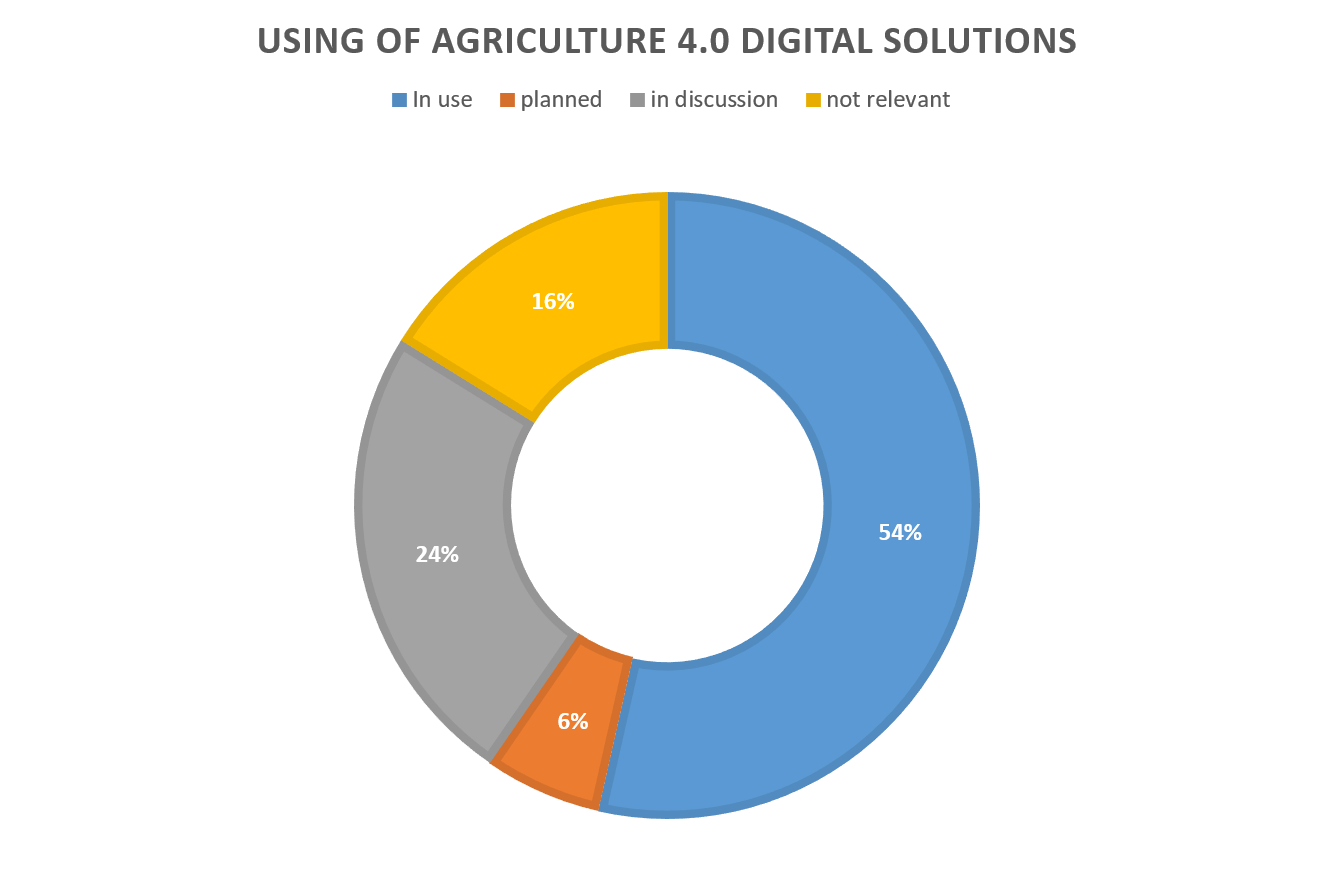
\includegraphics[width=1\columnwidth]{images/usingOfAgriculure4-0-solutions_pieChart}
\caption{Using of Agriculture 4.0 digital solutions}
\end{figure}

%TODO
%Quelle: Bitkom-Pressekonferenz-Digitalisierung-in-der-Landwirtschaft-02-11-2016-Praesentation

To get an initial impression of the \ac{IoT} progress and level of digitalisation in the agriculture industry, the figure above states out how many german companies in that industry are using and/or planning to use \ac{IoT} and digital solutions to optimize their agricultural business.

In general, smart farming and the use of \ac{IoT} technologies are increasing crop yields. Precise data about utilised agricultural area, weather and realtime tracking of active machines and systems are leading to higher food quality and more efficient use of ressources.

Challenges of the agriculture, forestry and fishing sector are linked to the ecological/climate change regarding consumer concerns and the globally increasing demand of food. \ac{I4.0} concepts are used to face those challenges.

\begin{figure}[H]
\centering
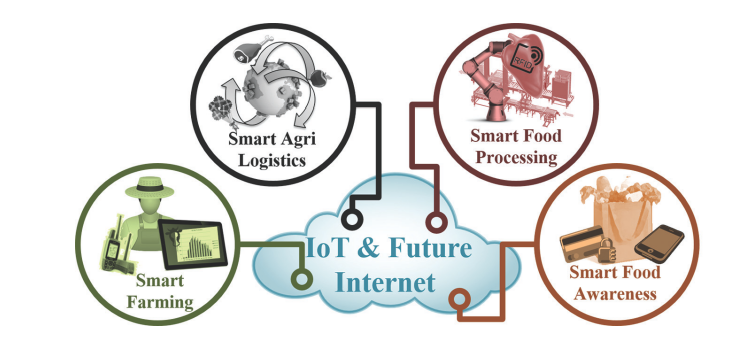
\includegraphics[width=1\columnwidth]{images/digitising-industry_agriculture_smartFarming}
\caption{Domains which are impacting this sector}
\end{figure}

%Quelle: Internet of Food and Farm 2020 p.133

Domains like smart farming, smart Agri-logistics, smart food processing and smart food awareness are used to describe the development of \ac{IoT} impact on the sector.




\subsection{Manufacturing}
The manufacturing sector is the most discussed sector in the literature. It is the focus sector of the \ac{I4.0} initiative and many companies such as McKinsey actually see \ac{I4.0} as a synonym for the digitalization of the manufacturing sector \cite[]{McKinseydigitizationIndustrialSector:2015}. Little beneficial advise can be given by us for this sector as it is being focused on by the \ac{I4.0} initiative itself and the suggestion should therefore be to follow this frameworks approaches as well as the \ac{IIC} publications regarding the cross sector specific interests \cite[]{iicarchitecture:2016}.

\subsection{Mining and quarrying; Electricity, gas, water supply and other industrial activities }

The sector of supplying basic utilities such as electricity, gas and water is a complex system in each vertical and horizontal level. Each level brings with it potentials and problems, but a generalized description is the task of finding a transportable base resource, extracting and delivering it to end consumers. The sector therefore requires extraction activities, industrial processing capabilities, supply chains and the \emph{"operation of transmission [and] distribution systems"}\cite[p. 166ff.]{ISIC:2008} for various utilities such as gas, electricity, water and others.

The electricity grid especially has been a focus of studies due to the politically demanded changes in energy sources and delivery \cite[p.12ff.]{AppelrathKagermannMayer2012}. Regarding the delivery of products that are not using a continuous delivery network such as the electricity or water supply grid, the recommendations by the \ac{WEF} that focus on logistics' improvement of efficiency and describe a \emph{"race to build a dominant global [logistics] platform"}\cite{worldforumlogistics:2016} can be applied. Regarding the industrial processing capabilities, again the \acf{I4.0Init} offers many guidelines and best practices.

The extraction of minerals in the form of mining and quarrying have been the focus by \citeauthor{mckinseymining:2015} who describe mining as a sector that has suffered from decreasing profitability due to a continuous price competition and competitors continuously improving their productivity. They imply that mining can greatly benefit from the classic building blocks of digitalization such as increased precision through sensors and downstream analytics to improve \emph{"material and equipment flow"} and create a \emph{"deeper understanding of the resource base"}. Automation, robotics and analytics can help improve efficiency and reduce downtime. Big improvement potentials become obvious when we look at the amount of data used for decision making which is a meager 1\% of the total data collected \cite[p.7]{mckinseymining:2015}.

Literature suggestions, aside from the works of the \ac{IIC} and \ac{I4.0Init} are therefore:

\begin{itemize}
\item Digital Transformation of Industries: Logistics \cite{worldforumlogistics:2016}
\item How digital innovation can improve mining productivity \cite{mckinseymining:2015}
\item Future Energy Grid: Migrationspfade ins Internet der Energie \cite{AppelrathKagermannMayer2012}
\end{itemize}


\subsection{Construction}
JO
%Quelle: Digitalisierung der Bauwirtschaft, Der europäische Weg zu "Construction 4.0", Roland Berger, 2016
%Quelle: Towards the next generation of intelligent building, Geriogius Lilis
%Quelle: Big Data in the construction industry, Muhammed Bilal
%Quelle: http://buildingsmart.org/about/vision-mission/core-purpose/

%TODO: Literatur fertig scannen und niederschreiben

According to a poll of the german chamber of Industry and Commerce (\ac{DIHK}) on March 2016, the sample of companies linked to the construction and building industry rate their level of Digitalisation on a scale from 1 to 6 as a 3,5, which is 0,2 points less than the average across all industries. This states out, that representers of the construction industry know, that they have future chances when they use digital Solutions and \ac{IoT}, but are not implementing those fast enough %TODO iteraturangabe DIHK Unternehmensbarometer

The \ac{IoT} impact on the construction or building industry is linked to terms like smart cities, lean construction management and smart resource management in construction processes. The main focus of Digitalisation processes in this domain is to reach higher levels of sustainability and energy efficiency %Quelle: Towards the next generation of intelligent building, Geriogius Lilis
Intelligent buildings are the transformational core in this industry. Regarding development in this industry facing the smart city topic, \ac{IoT} is very important and a leading driving force impacting the progress in development. Lean construction management and smart resource management is linked to more traditional construction progresses, so generally \ac{IoT} is used to expand innovation in those areas and is not transforming it itself.

Current examples of digital tools which support processes like planning, analysing, monitoring, and optimizing the construction of objects are e.g. the Building Information Modeling (\ac{BIM}) and also building automation systems (\ac{BAS}) which served the purpose reliably in the previous decades but need to be transformed to models, which cover \ac{IoT} progress and technological standards throughout integrating industries and operations. %Quelle: Towards the next generation of intelligent building, Giorgius Lilis

The \ac{BIM} and specifically the "Stufenplan Digitales Planen und Bauen" %TODO Quelle einpflegen
is a model which can be used to get digital processes involved in the industry regarding holistic perspectives or progresses. To get this in connection to the current impact of the Digitalisation on the industry, the "Bundesministerium für Verkehr und digitale Infrastruktur" makes the use of BIM mandatory for public infrastructural projects. %Quelle: Stufenplan Digitales Planen und Bauen

\ac{BAS} and building management systems \ac{BMS} are used to integrate many different data resources and construction processes to offer an "economy of large scale with expertise in the system control and automation engineering domains" %TODO Quote:G.Lilis et al./ Sustainable Cities and Society 28 (2017) p. 475
This states out, that these systems are being developed and are facing the challenges of Industry 4.0. On the other hand, the industries' best practices are legacy habits and relatively small innovation progress e.g. because of the close relationship to the public administration sector and administrative barriers.

In this paper, we can only state out general information about specific models, but the initiative "building smart" %TODO Link: http://buildingsmart.org/
and their so-called "international home of openBMI" is recommended to get further information regarding the assessment and status of Industry 4.0 progress in construction or building-industry focused business. Additionally we can recommend the BIMiD-reference-construction-process, which delivers an example of digitally planned construction project. % TODO Link http://www.bimid.de/aktuelles/bim-referenz-bau-prozess




\subsection{Wholesale and retail trade, transportation and storage, accommodation and food service activities}

This group is a collection of three sectors defined by \ac{ISIC}. The first sector, wholesale and retail trade, includes all \emph{"services incidental to the sale of [...] goods"}\cite[p.179]{ISIC:2008} as well as the specific task of motor vehicle repairs. The second sector, transportation and storage, includes all tasks related to logistics and storage of both objects and passengers.\cite[p.194]{ISIC:2008} The last one is focusing on the \emph{"short-stay accommodation for visitors"} as well as the \emph{"provision of complete meals and drinks fit for immediate consumption"}\cite[p.202]{ISIC:2008}

The second sector, transportation and storage, often also called logistics, offers large optimization potentials. As reported by \citeauthor{nytimesdrivingtruck:2016} in the New York Times, Uber, a digital pioneer in on-demand drive-hauling services, is actively working on autonomous trucks for logistics which has been demonstrated by an autonomously driving truck transporting goods 120 miles without the need of a driver in October 2016. Amazon recently introduced "intelligent" robots in their warehouses, greatly reducing the walking distances of "pickers", employees who collect products for orders. \cite{Kiva:amazon:Ma:2016:OTA:2936924.2937092}. Drones are being investigated as alternatives for delivering parcels and analytics can help fill many of empty trucks that can be up to 50\% of a fleet on their return trips \cite{worldforumlogistics:2016}.

The third sector, accomodation and food service activities, has already seen its fair share of digitalization fueled disruption with AirBnB disrupting the accomodation market and companies like foodora and deliveroo offering services aim to remove the location component of food services \cite{bloombergfoodora:2016}. Both are strategic markets that can be expected to stay, as long as humans eat, travel and sleep, but the model of serving these demands can differ greatly from current business models. Existing businesses need to challenge their business models and be willing to disrupt their own business to avoid competition from doing so.

For all three sectors in this group, the recommendations of the \ac{IIC} and \cite{I4.0Init} are valid. Especially the \ac{IIC} recommendations regarding vertical integrations of value chains in their architectural recommendations \cite{iicarchitecture:2016} are valuable for all three sectors due to their direct link with supply chains and logistic companies. In addition the following literature recommendations can be made:

\begin{itemize}
    \item The Business Model Navigator: 55 Models That Will Revolutionise Your Business \cite{gassmann2013geschaeftsmodelle}
    \item Leading Digital \cite{Leading Digital: Turning Technology Into Business Transformation}
    \item World Economic Forum White Paper Digital Transformation of Industries: Logistics Industry \cite{worldforumlogistics:2016}
\end{itemize}

\subsection{Information and Communication}
PB

\subsection{Financial and insurance activities}
JO
%TODO Literatur scannen und Quintessenz niederschreiben

The financial services industry, including financial service activities, Insurance, reinsurance, pension funding and activities auxiliary to Financial and insurance activities \citeauthor{ISIC:2008} are facing transformation throughout digitalisation processes. The final Report of the \ac{WEF} addresses the future of Financial Services regarding the impact of disruptive innovations and \ac{IoT} \citeauthor{WEF-futureFinancialServices} and is dividing the financial services industry into 6 functions and 11 Clusters of Innovation, which are influencing and are influenced by disruptive innovations and digitalisation progress.
The functions are:
Payments, Insurance, Deposits \& Lending, Capital Raising, Investment Management, Market Provisioning

The clusters of Innovation are:
Emerging Payment Rails, Cashless World, Insurance Disaggregation, Connected Insurance, Alternative Lending, Shifting Customer Preferences, Crowdfunding, Empowered Investors, Process Externalisation, New Market Platforms, Smarter \& faster Machines.

%TODO Grafik entfernen
\begin{figure}[H]
\centering
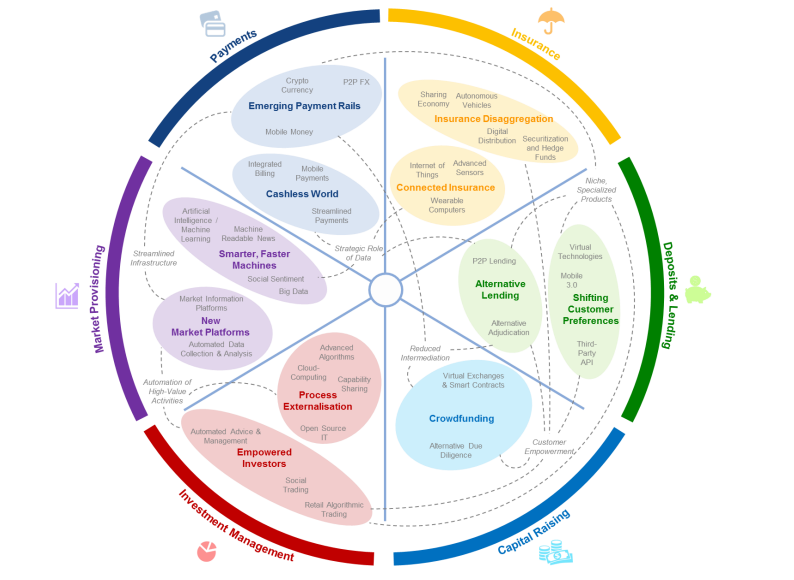
\includegraphics[width=1\columnwidth]{images/industry-financial-services-6segments_wef-copyright.PNG}
\caption{6 functions and 11 Clusters of innovation in the financial services industry}
\end{figure}

Furthermore, the progress in several functions is currently shaping new business opportunities, e.g. Fintech start-ups or more integrated business processes which are generating more values for the economy and the requirements of the society.
Typical barriers of the industry and the implementation of innovations like \ac{IoT} are Accountability, Privacy, Security, Interoperability and Reliability. \cite{WEF-futureFinancialServices, Weber2011133, CapGemini-IoT-financialServices} %TODO Literaturhinweis überprüfen

The pressure of innovating legacy processes in this industry is already latent. To get profound results, the transformation requires changes in areas, which are linked to each other. Therefore, integration is elementary for success. As it is stated out in the paper of \citeauthor{ArthurDLittle-FinancialService} "The transformation normally requires important changes in processes, organization structure, and company systems, and must involve all business and IT areas" \cite[p.4 ]{ArthurDLittle-FinancialService}. Accenture's \emph{European Financial Services Digital Readiness Report} also confirms, that financial services firms need to change their processes all over the their organization across the four core business areas plan, make, sell and manage. \cite[p. 9]{accenture-europeanFinancialServices-digitalReadinessReport}

Regarding these profound changes in the financial and insurance activities, it has to be stated out, if the IIC and I4.0 Frameworks can be applicable to accomplish the progress. The \ac{RAMI} itself is a good starting point for the financial services industry, but cannot outline specific challenges and conditions of that industry. Extending those general frameworks with more detailed actions is recommended. Following Frameworks can be used:


\subsection{Real estate activities}
JO
%TODO noch Literatur recherchieren

Companies in the real estate industry face several similar challenges like the construction industry. Other activities, like the real-estate broker or property management can use \ac{IoT} to automate monitoring current status of real estate objects or energy supply on the spot.

\subsection{Professional, scientific, technical, administrative and support service activities}
%PB

Professional services such as legal support, administration, engineering and architecture are affected very little by the effects of digitalization and industry 4.0 in the sense that they aren't the ones getting digitalised but rather are the ones pushing forward this transformation. It is therefore not logical to apply \ac{I4.0} concepts to this sector, however it is important for those professionals to be knowledgeable about the factors of it since they are major players regarding its planning and implementation. They should therefore have a broad high level knowledge about the overall trend with specialized knowledge for their focus industries.

In the phase of designing the \ac{DT} there are many relevant topics. Managing roles focus on the planning and controlling of the business branches and activities. Such tasks can greatly benefit from knowledge derived from the information exposed through sensors and analysed with tools from data science enabling \emph{"real-time business and operational decisions"} \cite[p.84]{iicarchitecture:2016}.

There are also big aspects such as security, governance and controlling activities that can benefit from the \ac{DT}. As \citeauthor{Tragos2016trusted} note, The \ac{IoT} leads to many unnoticeable devices spread around public places that monitor and log a variety of information which can be considered a necessary tool but also a source of privacy invasion. Strong security measures need to be deployed to ensure all dimensions of the \emph{\ac{IoT} trustworthiness} are covered which are explained in detail by the \ac{IIC} in their Security Framework \cite{iicsecurity:2016}.

\begin{figure}[H]
\centering
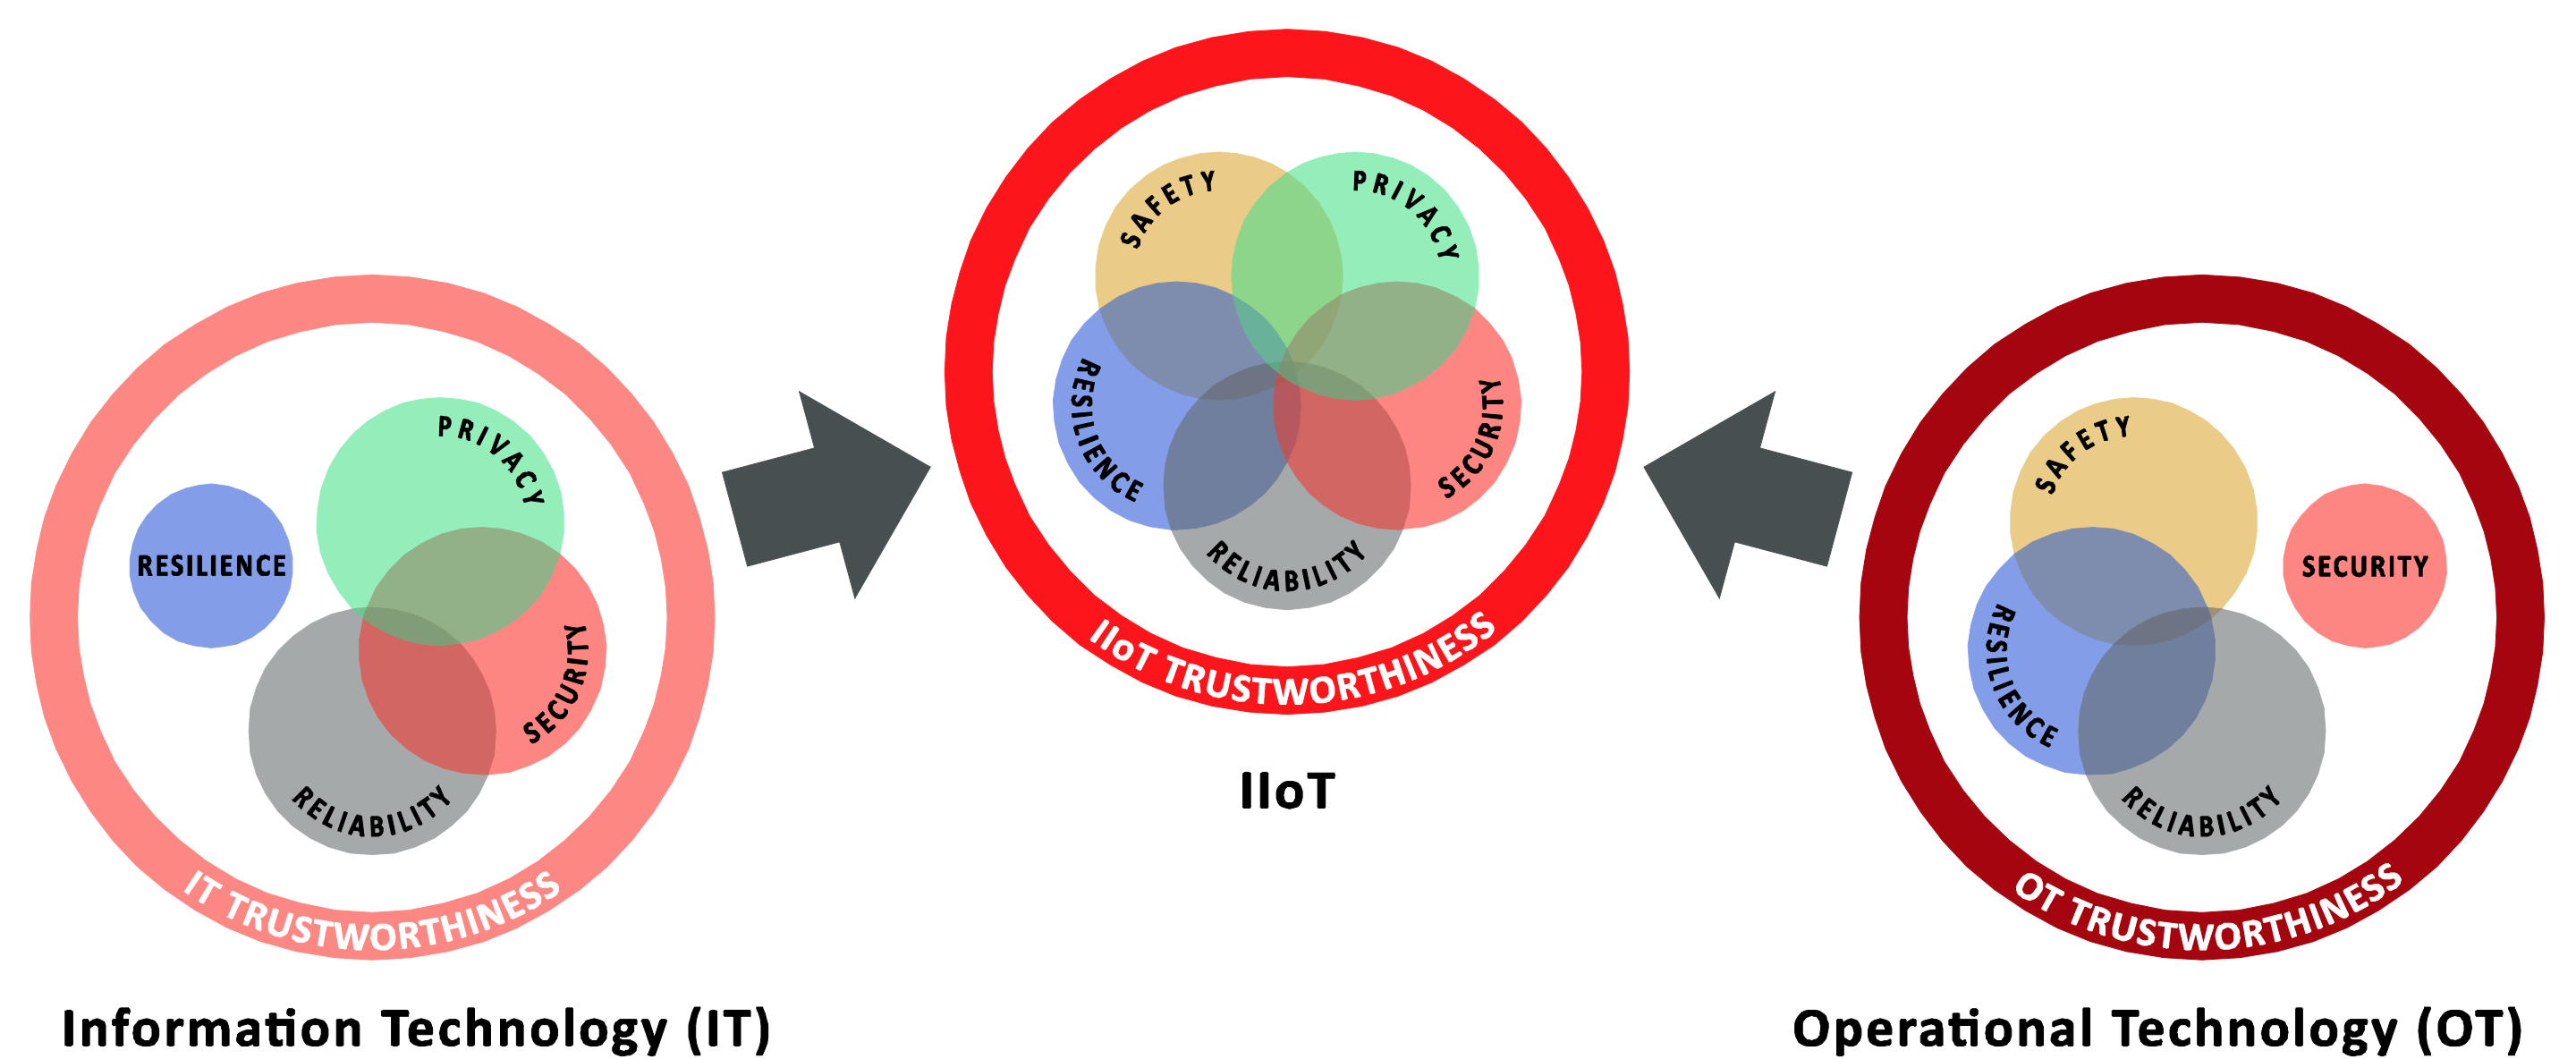
\includegraphics[width=1\columnwidth]{images/iic-iiot-trustworthiness}
\caption{\ac{IIC} Security Framework}
\end{figure}

To summarise, the sector is a major player in the design of the \ac{DT} but is not directly affected by it in the sense of it being the subject of transformation. Professionals and businesses in this sector are therefore advised to build up knowledge about the \ac{DT} and familiarise themselves with the core concepts of \ac{I4.0}. The two frameworks by the \ac{IIC} and the \ac{I4.0} initiative are an excellent guideline for this.

\subsection{Public administration and defence, education, human health and social work activities}
PB
%JO TODO habe ein gutes Uebersicht Paper fuer dich gefunden. Siehe Dropbox Literatur Ordner #healthcare-industry

\subsection{Other service activities}
%JO
The \ac{ISIC} defines this sector as a residual category including membership organizations, repair services for personal equipment as well as cleaning and beauty services \cite[p.262ff.]{ISIC:2008}.

These categories of economic activity, aside from the membership organizations, are composed mainly of small to medium size businesses. Such businesses rarely have the capacity to compose a complex implementation of a digitalization strategy which causes the \ac{I4.0Init} and \ac{IIC} frameworks to be inadequate.

A non-technical and

JO! SWitch
